\documentclass[twoside]{book}

% Packages required by doxygen
\usepackage{fixltx2e}
\usepackage{calc}
\usepackage{doxygen}
\usepackage[export]{adjustbox} % also loads graphicx
\usepackage{graphicx}
\usepackage[utf8]{inputenc}
\usepackage{makeidx}
\usepackage{multicol}
\usepackage{multirow}
\PassOptionsToPackage{warn}{textcomp}
\usepackage{textcomp}
\usepackage[nointegrals]{wasysym}
\usepackage[table]{xcolor}

% Font selection
\usepackage[T1]{fontenc}
\usepackage[scaled=.90]{helvet}
\usepackage{courier}
\usepackage{amssymb}
\usepackage{sectsty}
\renewcommand{\familydefault}{\sfdefault}
\allsectionsfont{%
  \fontseries{bc}\selectfont%
  \color{darkgray}%
}
\renewcommand{\DoxyLabelFont}{%
  \fontseries{bc}\selectfont%
  \color{darkgray}%
}
\newcommand{\+}{\discretionary{\mbox{\scriptsize$\hookleftarrow$}}{}{}}

% Page & text layout
\usepackage{geometry}
\geometry{%
  a4paper,%
  top=2.5cm,%
  bottom=2.5cm,%
  left=2.5cm,%
  right=2.5cm%
}
\tolerance=750
\hfuzz=15pt
\hbadness=750
\setlength{\emergencystretch}{15pt}
\setlength{\parindent}{0cm}
\setlength{\parskip}{3ex plus 2ex minus 2ex}
\makeatletter
\renewcommand{\paragraph}{%
  \@startsection{paragraph}{4}{0ex}{-1.0ex}{1.0ex}{%
    \normalfont\normalsize\bfseries\SS@parafont%
  }%
}
\renewcommand{\subparagraph}{%
  \@startsection{subparagraph}{5}{0ex}{-1.0ex}{1.0ex}{%
    \normalfont\normalsize\bfseries\SS@subparafont%
  }%
}
\makeatother

% Headers & footers
\usepackage{fancyhdr}
\pagestyle{fancyplain}
\fancyhead[LE]{\fancyplain{}{\bfseries\thepage}}
\fancyhead[CE]{\fancyplain{}{}}
\fancyhead[RE]{\fancyplain{}{\bfseries\leftmark}}
\fancyhead[LO]{\fancyplain{}{\bfseries\rightmark}}
\fancyhead[CO]{\fancyplain{}{}}
\fancyhead[RO]{\fancyplain{}{\bfseries\thepage}}
\fancyfoot[LE]{\fancyplain{}{}}
\fancyfoot[CE]{\fancyplain{}{}}
\fancyfoot[RE]{\fancyplain{}{\bfseries\scriptsize Generated by Doxygen }}
\fancyfoot[LO]{\fancyplain{}{\bfseries\scriptsize Generated by Doxygen }}
\fancyfoot[CO]{\fancyplain{}{}}
\fancyfoot[RO]{\fancyplain{}{}}
\renewcommand{\footrulewidth}{0.4pt}
\renewcommand{\chaptermark}[1]{%
  \markboth{#1}{}%
}
\renewcommand{\sectionmark}[1]{%
  \markright{\thesection\ #1}%
}

% Indices & bibliography
\usepackage{natbib}
\usepackage[titles]{tocloft}
\setcounter{tocdepth}{3}
\setcounter{secnumdepth}{5}
\makeindex

% Hyperlinks (required, but should be loaded last)
\usepackage{ifpdf}
\ifpdf
  \usepackage[pdftex,pagebackref=true]{hyperref}
\else
  \usepackage[ps2pdf,pagebackref=true]{hyperref}
\fi
\hypersetup{%
  colorlinks=true,%
  linkcolor=blue,%
  citecolor=blue,%
  unicode%
}

% Custom commands
\newcommand{\clearemptydoublepage}{%
  \newpage{\pagestyle{empty}\cleardoublepage}%
}

\usepackage{caption}
\captionsetup{labelsep=space,justification=centering,font={bf},singlelinecheck=off,skip=4pt,position=top}

%===== C O N T E N T S =====

\begin{document}

% Titlepage & ToC
\hypersetup{pageanchor=false,
             bookmarksnumbered=true,
             pdfencoding=unicode
            }
\pagenumbering{alph}
\begin{titlepage}
\vspace*{7cm}
\begin{center}%
{\Large Numerical Integration }\\
\vspace*{1cm}
{\large Generated by Doxygen 1.8.13}\\
\end{center}
\end{titlepage}
\clearemptydoublepage
\pagenumbering{roman}
\tableofcontents
\clearemptydoublepage
\pagenumbering{arabic}
\hypersetup{pageanchor=true}

%--- Begin generated contents ---
\chapter{Hierarchical Index}
\section{Class Hierarchy}
This inheritance list is sorted roughly, but not completely, alphabetically\+:\begin{DoxyCompactList}
\item \contentsline{section}{Abstract\+Integral\+Solver$<$ t $>$}{\pageref{class_abstract_integral_solver}}{}
\item \contentsline{section}{Abstract\+Integral\+Solver$<$ std\+:\+:function$<$ double(double)$>$ $>$}{\pageref{class_abstract_integral_solver}}{}
\begin{DoxyCompactList}
\item \contentsline{section}{Abstract1\+D\+Integral\+Solver}{\pageref{class_abstract1_d_integral_solver}}{}
\begin{DoxyCompactList}
\item \contentsline{section}{Mid\+Point\+Solver}{\pageref{class_mid_point_solver}}{}
\item \contentsline{section}{Simpson\+Solver}{\pageref{class_simpson_solver}}{}
\item \contentsline{section}{Trapez\+Solver}{\pageref{class_trapez_solver}}{}
\end{DoxyCompactList}
\end{DoxyCompactList}
\item \contentsline{section}{Abstract\+Integral\+Solver$<$ std\+:\+:function$<$ double(double, double)$>$ $>$}{\pageref{class_abstract_integral_solver}}{}
\begin{DoxyCompactList}
\item \contentsline{section}{Abstract2\+D\+Integral\+Solver}{\pageref{class_abstract2_d_integral_solver}}{}
\begin{DoxyCompactList}
\item \contentsline{section}{Mid\+Point2\+D\+Solver}{\pageref{class_mid_point2_d_solver}}{}
\item \contentsline{section}{Simpson2\+D\+Solver}{\pageref{class_simpson2_d_solver}}{}
\item \contentsline{section}{Trapez2\+D\+Solver}{\pageref{class_trapez2_d_solver}}{}
\end{DoxyCompactList}
\end{DoxyCompactList}
\item \contentsline{section}{test\+Suite1D}{\pageref{classtest_suite1_d}}{}
\end{DoxyCompactList}

\chapter{Class Index}
\section{Class List}
Here are the classes, structs, unions and interfaces with brief descriptions\+:\begin{DoxyCompactList}
\item\contentsline{section}{\hyperlink{class_abstract1_d_integral_solver}{Abstract1\+D\+Integral\+Solver} }{\pageref{class_abstract1_d_integral_solver}}{}
\item\contentsline{section}{\hyperlink{class_abstract2_d_integral_solver}{Abstract2\+D\+Integral\+Solver} }{\pageref{class_abstract2_d_integral_solver}}{}
\item\contentsline{section}{\hyperlink{class_abstract_integral_solver}{Abstract\+Integral\+Solver$<$ t $>$} }{\pageref{class_abstract_integral_solver}}{}
\item\contentsline{section}{\hyperlink{class_mid_point2_d_solver}{Mid\+Point2\+D\+Solver} }{\pageref{class_mid_point2_d_solver}}{}
\item\contentsline{section}{\hyperlink{class_mid_point_solver}{Mid\+Point\+Solver} }{\pageref{class_mid_point_solver}}{}
\item\contentsline{section}{\hyperlink{class_simpson2_d_solver}{Simpson2\+D\+Solver} }{\pageref{class_simpson2_d_solver}}{}
\item\contentsline{section}{\hyperlink{class_simpson_solver}{Simpson\+Solver} }{\pageref{class_simpson_solver}}{}
\item\contentsline{section}{\hyperlink{class_trapez2_d_solver}{Trapez2\+D\+Solver} }{\pageref{class_trapez2_d_solver}}{}
\item\contentsline{section}{\hyperlink{class_trapez_solver}{Trapez\+Solver} }{\pageref{class_trapez_solver}}{}
\end{DoxyCompactList}

\chapter{Class Documentation}
\hypertarget{class_abstract1_d_integral_solver}{}\section{Abstract1\+D\+Integral\+Solver Class Reference}
\label{class_abstract1_d_integral_solver}\index{Abstract1\+D\+Integral\+Solver@{Abstract1\+D\+Integral\+Solver}}


Inheritance diagram for Abstract1\+D\+Integral\+Solver\+:
\nopagebreak
\begin{figure}[H]
\begin{center}
\leavevmode
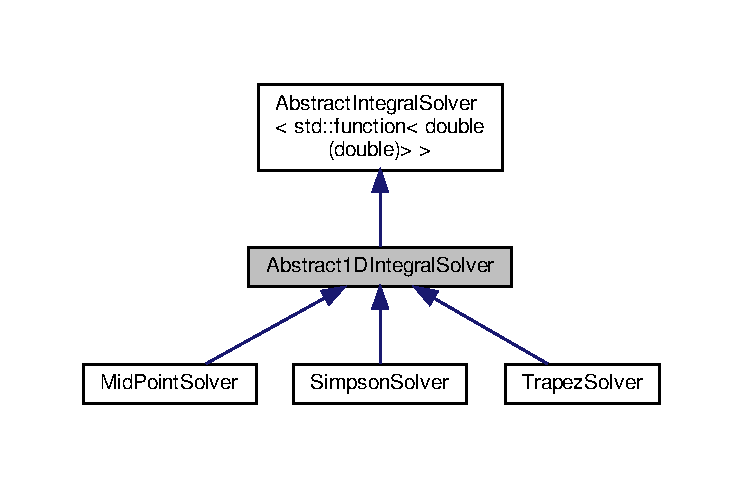
\includegraphics[width=350pt]{class_abstract1_d_integral_solver__inherit__graph}
\end{center}
\end{figure}


Collaboration diagram for Abstract1\+D\+Integral\+Solver\+:
\nopagebreak
\begin{figure}[H]
\begin{center}
\leavevmode
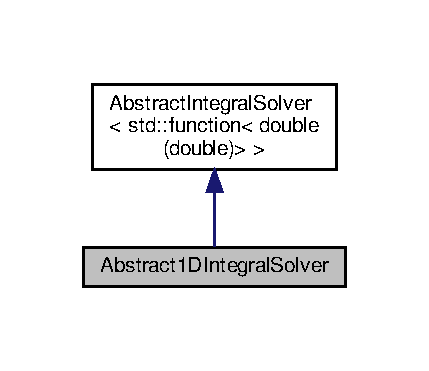
\includegraphics[width=206pt]{class_abstract1_d_integral_solver__coll__graph}
\end{center}
\end{figure}
\subsection*{Public Types}
\begin{DoxyCompactItemize}
\item 
\mbox{\Hypertarget{class_abstract1_d_integral_solver_a7d8e60dfe7eb70e5c19dd71ac0b03880}\label{class_abstract1_d_integral_solver_a7d8e60dfe7eb70e5c19dd71ac0b03880}} 
using {\bfseries t} = std\+::function$<$ double(double)$>$
\end{DoxyCompactItemize}
\subsection*{Public Member Functions}
\begin{DoxyCompactItemize}
\item 
\mbox{\Hypertarget{class_abstract1_d_integral_solver_aff8ede805704db176953095b7578db37}\label{class_abstract1_d_integral_solver_aff8ede805704db176953095b7578db37}} 
{\bfseries Abstract1\+D\+Integral\+Solver} (int n, double x0, double xf, t f)
\end{DoxyCompactItemize}
\subsection*{Additional Inherited Members}


The documentation for this class was generated from the following file\+:\begin{DoxyCompactItemize}
\item 
Abstract1\+D\+Integral\+Solver.\+h\end{DoxyCompactItemize}

\hypertarget{class_abstract2_d_integral_solver}{}\section{Abstract2\+D\+Integral\+Solver Class Reference}
\label{class_abstract2_d_integral_solver}\index{Abstract2\+D\+Integral\+Solver@{Abstract2\+D\+Integral\+Solver}}


{\ttfamily \#include $<$Abstract2\+D\+Integral\+Solver.\+hpp$>$}



Inheritance diagram for Abstract2\+D\+Integral\+Solver\+:\nopagebreak
\begin{figure}[H]
\begin{center}
\leavevmode
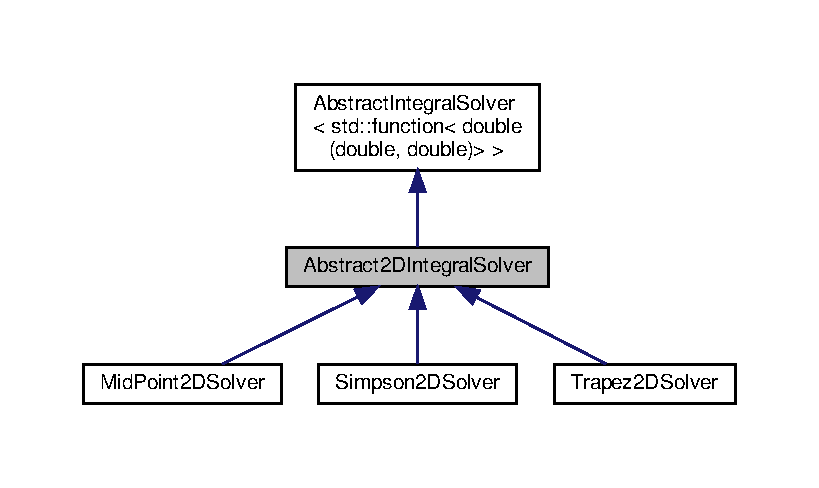
\includegraphics[width=350pt]{class_abstract2_d_integral_solver__inherit__graph}
\end{center}
\end{figure}


Collaboration diagram for Abstract2\+D\+Integral\+Solver\+:\nopagebreak
\begin{figure}[H]
\begin{center}
\leavevmode
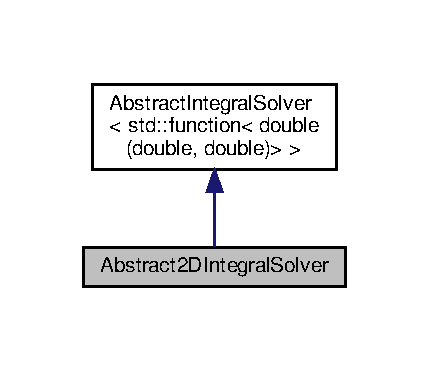
\includegraphics[width=206pt]{class_abstract2_d_integral_solver__coll__graph}
\end{center}
\end{figure}
\subsection*{Public Types}
\begin{DoxyCompactItemize}
\item 
using \hyperlink{class_abstract2_d_integral_solver_ab660df32953c6b0f9f3a45a8720eaeb3}{t} = \hyperlink{_tests_8cpp_a1c2dbde1ba7d93e381d4ccb9f603be16}{std\+::function}$<$ double(double, double)$>$
\end{DoxyCompactItemize}
\subsection*{Public Member Functions}
\begin{DoxyCompactItemize}
\item 
\hyperlink{class_abstract2_d_integral_solver_ad25b34f07befbbad7d3ec2b76d47b2b7}{Abstract2\+D\+Integral\+Solver} (int n\+\_\+x, double x0, double xf, int n\+\_\+y, double y0, double yf, \hyperlink{class_abstract2_d_integral_solver_ab660df32953c6b0f9f3a45a8720eaeb3}{t} f)
\item 
double \hyperlink{class_abstract2_d_integral_solver_a925351cc0ac65900e7ff42fd9d7e6973}{Get\+Function\+Value} (double x, double y) const
\item 
double \hyperlink{class_abstract2_d_integral_solver_a337907e938e5aa286618fd582b7b304e}{Get\+Initial\+Argument\+\_\+y} () const
\item 
double \hyperlink{class_abstract2_d_integral_solver_ab4a24610598fa26556c60c449d757b65}{Get\+Final\+Argument\+\_\+y} () const
\item 
double \hyperlink{class_abstract2_d_integral_solver_ad82316695f57ad589714598617c7784d}{Get\+Number\+Of\+Steps\+\_\+y} () const
\item 
double \hyperlink{class_abstract2_d_integral_solver_a5c23a838a4db9b607140d4d5f03b4f79}{Get\+Step\+Size\+\_\+y} () const
\end{DoxyCompactItemize}
\subsection*{Additional Inherited Members}


\subsection{Detailed Description}
\hyperlink{class_abstract2_d_integral_solver}{Abstract2\+D\+Integral\+Solver} is the abstract mother class for 2D integral solvers. It defines a new constructor for 2D integrals, the necessary methods in the y direction and the type of the function 

\subsection{Member Typedef Documentation}
\mbox{\Hypertarget{class_abstract2_d_integral_solver_ab660df32953c6b0f9f3a45a8720eaeb3}\label{class_abstract2_d_integral_solver_ab660df32953c6b0f9f3a45a8720eaeb3}} 
\index{Abstract2\+D\+Integral\+Solver@{Abstract2\+D\+Integral\+Solver}!t@{t}}
\index{t@{t}!Abstract2\+D\+Integral\+Solver@{Abstract2\+D\+Integral\+Solver}}
\subsubsection{\texorpdfstring{t}{t}}
{\footnotesize\ttfamily using \hyperlink{class_abstract2_d_integral_solver_ab660df32953c6b0f9f3a45a8720eaeb3}{Abstract2\+D\+Integral\+Solver\+::t} =  \hyperlink{_tests_8cpp_a1c2dbde1ba7d93e381d4ccb9f603be16}{std\+::function}$<$double(double, double)$>$}

namespace t is defined as a function which takes two double as arguments and returns a double. 

\subsection{Constructor \& Destructor Documentation}
\mbox{\Hypertarget{class_abstract2_d_integral_solver_ad25b34f07befbbad7d3ec2b76d47b2b7}\label{class_abstract2_d_integral_solver_ad25b34f07befbbad7d3ec2b76d47b2b7}} 
\index{Abstract2\+D\+Integral\+Solver@{Abstract2\+D\+Integral\+Solver}!Abstract2\+D\+Integral\+Solver@{Abstract2\+D\+Integral\+Solver}}
\index{Abstract2\+D\+Integral\+Solver@{Abstract2\+D\+Integral\+Solver}!Abstract2\+D\+Integral\+Solver@{Abstract2\+D\+Integral\+Solver}}
\subsubsection{\texorpdfstring{Abstract2\+D\+Integral\+Solver()}{Abstract2DIntegralSolver()}}
{\footnotesize\ttfamily Abstract2\+D\+Integral\+Solver\+::\+Abstract2\+D\+Integral\+Solver (\begin{DoxyParamCaption}\item[{int}]{n\+\_\+x,  }\item[{double}]{x0,  }\item[{double}]{xf,  }\item[{int}]{n\+\_\+y,  }\item[{double}]{y0,  }\item[{double}]{yf,  }\item[{\hyperlink{class_abstract2_d_integral_solver_ab660df32953c6b0f9f3a45a8720eaeb3}{t}}]{f }\end{DoxyParamCaption})}

New constructor for 2D integrals 
\begin{DoxyParams}{Parameters}
{\em n\+\_\+x} & the number of steps in the x direction \\
\hline
{\em x0} & the beginning of the x interval \\
\hline
{\em xf} & the end of the x interval \\
\hline
{\em n\+\_\+y} & the number of steps in the y direction \\
\hline
{\em y0} & the beginning of the y interval \\
\hline
{\em yf} & the end of the y interval \\
\hline
{\em f} & the function dependent on x and y \\
\hline
\end{DoxyParams}


\subsection{Member Function Documentation}
\mbox{\Hypertarget{class_abstract2_d_integral_solver_ab4a24610598fa26556c60c449d757b65}\label{class_abstract2_d_integral_solver_ab4a24610598fa26556c60c449d757b65}} 
\index{Abstract2\+D\+Integral\+Solver@{Abstract2\+D\+Integral\+Solver}!Get\+Final\+Argument\+\_\+y@{Get\+Final\+Argument\+\_\+y}}
\index{Get\+Final\+Argument\+\_\+y@{Get\+Final\+Argument\+\_\+y}!Abstract2\+D\+Integral\+Solver@{Abstract2\+D\+Integral\+Solver}}
\subsubsection{\texorpdfstring{Get\+Final\+Argument\+\_\+y()}{GetFinalArgument\_y()}}
{\footnotesize\ttfamily double Abstract2\+D\+Integral\+Solver\+::\+Get\+Final\+Argument\+\_\+y (\begin{DoxyParamCaption}{ }\end{DoxyParamCaption}) const\hspace{0.3cm}{\ttfamily [inline]}}

Method to access to the end of the y interval \begin{DoxyReturn}{Returns}
the final y argument 
\end{DoxyReturn}
\mbox{\Hypertarget{class_abstract2_d_integral_solver_a925351cc0ac65900e7ff42fd9d7e6973}\label{class_abstract2_d_integral_solver_a925351cc0ac65900e7ff42fd9d7e6973}} 
\index{Abstract2\+D\+Integral\+Solver@{Abstract2\+D\+Integral\+Solver}!Get\+Function\+Value@{Get\+Function\+Value}}
\index{Get\+Function\+Value@{Get\+Function\+Value}!Abstract2\+D\+Integral\+Solver@{Abstract2\+D\+Integral\+Solver}}
\subsubsection{\texorpdfstring{Get\+Function\+Value()}{GetFunctionValue()}}
{\footnotesize\ttfamily double Abstract2\+D\+Integral\+Solver\+::\+Get\+Function\+Value (\begin{DoxyParamCaption}\item[{double}]{x,  }\item[{double}]{y }\end{DoxyParamCaption}) const\hspace{0.3cm}{\ttfamily [inline]}}

Method to get the value of the function 
\begin{DoxyParams}{Parameters}
{\em x} & the x argument \\
\hline
{\em y} & the y argument \\
\hline
\end{DoxyParams}
\begin{DoxyReturn}{Returns}
the value of the funxtion at x and y 
\end{DoxyReturn}
\mbox{\Hypertarget{class_abstract2_d_integral_solver_a337907e938e5aa286618fd582b7b304e}\label{class_abstract2_d_integral_solver_a337907e938e5aa286618fd582b7b304e}} 
\index{Abstract2\+D\+Integral\+Solver@{Abstract2\+D\+Integral\+Solver}!Get\+Initial\+Argument\+\_\+y@{Get\+Initial\+Argument\+\_\+y}}
\index{Get\+Initial\+Argument\+\_\+y@{Get\+Initial\+Argument\+\_\+y}!Abstract2\+D\+Integral\+Solver@{Abstract2\+D\+Integral\+Solver}}
\subsubsection{\texorpdfstring{Get\+Initial\+Argument\+\_\+y()}{GetInitialArgument\_y()}}
{\footnotesize\ttfamily double Abstract2\+D\+Integral\+Solver\+::\+Get\+Initial\+Argument\+\_\+y (\begin{DoxyParamCaption}{ }\end{DoxyParamCaption}) const\hspace{0.3cm}{\ttfamily [inline]}}

Method to access to the beginning of the y interval \begin{DoxyReturn}{Returns}
the initial y argument 
\end{DoxyReturn}
\mbox{\Hypertarget{class_abstract2_d_integral_solver_ad82316695f57ad589714598617c7784d}\label{class_abstract2_d_integral_solver_ad82316695f57ad589714598617c7784d}} 
\index{Abstract2\+D\+Integral\+Solver@{Abstract2\+D\+Integral\+Solver}!Get\+Number\+Of\+Steps\+\_\+y@{Get\+Number\+Of\+Steps\+\_\+y}}
\index{Get\+Number\+Of\+Steps\+\_\+y@{Get\+Number\+Of\+Steps\+\_\+y}!Abstract2\+D\+Integral\+Solver@{Abstract2\+D\+Integral\+Solver}}
\subsubsection{\texorpdfstring{Get\+Number\+Of\+Steps\+\_\+y()}{GetNumberOfSteps\_y()}}
{\footnotesize\ttfamily double Abstract2\+D\+Integral\+Solver\+::\+Get\+Number\+Of\+Steps\+\_\+y (\begin{DoxyParamCaption}{ }\end{DoxyParamCaption}) const\hspace{0.3cm}{\ttfamily [inline]}}

Method to access to the number of steps used in y direction \begin{DoxyReturn}{Returns}
the number of steps in y direction 
\end{DoxyReturn}
\mbox{\Hypertarget{class_abstract2_d_integral_solver_a5c23a838a4db9b607140d4d5f03b4f79}\label{class_abstract2_d_integral_solver_a5c23a838a4db9b607140d4d5f03b4f79}} 
\index{Abstract2\+D\+Integral\+Solver@{Abstract2\+D\+Integral\+Solver}!Get\+Step\+Size\+\_\+y@{Get\+Step\+Size\+\_\+y}}
\index{Get\+Step\+Size\+\_\+y@{Get\+Step\+Size\+\_\+y}!Abstract2\+D\+Integral\+Solver@{Abstract2\+D\+Integral\+Solver}}
\subsubsection{\texorpdfstring{Get\+Step\+Size\+\_\+y()}{GetStepSize\_y()}}
{\footnotesize\ttfamily double Abstract2\+D\+Integral\+Solver\+::\+Get\+Step\+Size\+\_\+y (\begin{DoxyParamCaption}{ }\end{DoxyParamCaption}) const\hspace{0.3cm}{\ttfamily [inline]}}

Method to calculate the step size in y direction which is function of the interval and the number of steps \begin{DoxyReturn}{Returns}
the step size in y direction 
\end{DoxyReturn}


The documentation for this class was generated from the following files\+:\begin{DoxyCompactItemize}
\item 
\hyperlink{_abstract2_d_integral_solver_8hpp}{Abstract2\+D\+Integral\+Solver.\+hpp}\item 
\hyperlink{_abstract2_d_integral_solver_8cpp}{Abstract2\+D\+Integral\+Solver.\+cpp}\end{DoxyCompactItemize}

\hypertarget{class_abstract_integral_solver}{}\section{Abstract\+Integral\+Solver$<$ t $>$ Class Template Reference}
\label{class_abstract_integral_solver}\index{Abstract\+Integral\+Solver$<$ t $>$@{Abstract\+Integral\+Solver$<$ t $>$}}


{\ttfamily \#include $<$Abstract\+Integral\+Solver.\+hpp$>$}



Collaboration diagram for Abstract\+Integral\+Solver$<$ t $>$\+:\nopagebreak
\begin{figure}[H]
\begin{center}
\leavevmode
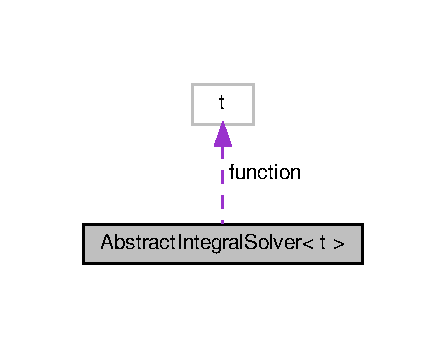
\includegraphics[width=214pt]{class_abstract_integral_solver__coll__graph}
\end{center}
\end{figure}
\subsection*{Public Member Functions}
\begin{DoxyCompactItemize}
\item 
\hyperlink{class_abstract_integral_solver_a44d64706b428c7b0bd4c9779c4d32b6f}{Abstract\+Integral\+Solver} (int number\+Of\+Steps, double initial\+Argument, double final\+Argument, t \hyperlink{class_abstract_integral_solver_ae31c391a21c6057e313295ad04de8a69}{function})
\item 
void \hyperlink{class_abstract_integral_solver_ab74cb9894daf3bcc97e14158a6087d99}{Set\+Number\+Of\+Steps} (const double n)
\item 
void \hyperlink{class_abstract_integral_solver_a891baae0103a8b488cf6cd007c109844}{Set\+Interval} (double x0, double xf)
\item 
void \hyperlink{class_abstract_integral_solver_adfb6eb8d70ebaf103e25ce468ac38b40}{Set\+Function} (t f)
\item 
{\footnotesize template$<$typename param $>$ }\\double \hyperlink{class_abstract_integral_solver_ae2f3d78fabe31ebe3b328fb6c52a2209}{Get\+Function\+Value} (param x) const
\item 
virtual double \hyperlink{class_abstract_integral_solver_ad87cb44c5ef3122bc95be48f473ba399}{Solve\+Integral} ()=0
\item 
double \hyperlink{class_abstract_integral_solver_adb8ef30d8231a173ee85e91155829daa}{Get\+Initial\+Argument} () const
\item 
double \hyperlink{class_abstract_integral_solver_a30f25ec2dff6d5881875952bec1d1774}{Get\+Final\+Argument} () const
\item 
double \hyperlink{class_abstract_integral_solver_a90148ecbeb6396638c428a319a7031dd}{Get\+Number\+Of\+Steps} () const
\item 
double \hyperlink{class_abstract_integral_solver_a0220c77810a813699748b875627da1a7}{Get\+Step\+Size} () const
\end{DoxyCompactItemize}
\subsection*{Public Attributes}
\begin{DoxyCompactItemize}
\item 
t \hyperlink{class_abstract_integral_solver_ae31c391a21c6057e313295ad04de8a69}{function}
\end{DoxyCompactItemize}


\subsection{Detailed Description}
\subsubsection*{template$<$typename t$>$\newline
class Abstract\+Integral\+Solver$<$ t $>$}


\begin{DoxyTemplParams}{Template Parameters}
{\em t} & \hyperlink{class_abstract_integral_solver}{Abstract\+Integral\+Solver} is the abstract mother class for 1D and 2D abstract integral solvers. It provides a basic constructor as well as methods that are common for both 1D and 2D numerical solvers. In order to provide polymorphism to accept both 1D and 2D functions, this is a templated class. \\
\hline
\end{DoxyTemplParams}


\subsection{Constructor \& Destructor Documentation}
\mbox{\Hypertarget{class_abstract_integral_solver_a44d64706b428c7b0bd4c9779c4d32b6f}\label{class_abstract_integral_solver_a44d64706b428c7b0bd4c9779c4d32b6f}} 
\index{Abstract\+Integral\+Solver@{Abstract\+Integral\+Solver}!Abstract\+Integral\+Solver@{Abstract\+Integral\+Solver}}
\index{Abstract\+Integral\+Solver@{Abstract\+Integral\+Solver}!Abstract\+Integral\+Solver@{Abstract\+Integral\+Solver}}
\subsubsection{\texorpdfstring{Abstract\+Integral\+Solver()}{AbstractIntegralSolver()}}
{\footnotesize\ttfamily template$<$typename t$>$ \\
\hyperlink{class_abstract_integral_solver}{Abstract\+Integral\+Solver}$<$ t $>$\+::\hyperlink{class_abstract_integral_solver}{Abstract\+Integral\+Solver} (\begin{DoxyParamCaption}\item[{int}]{number\+Of\+Steps,  }\item[{double}]{initial\+Argument,  }\item[{double}]{final\+Argument,  }\item[{t}]{function }\end{DoxyParamCaption})}

Constructor with every necessary argument 
\begin{DoxyParams}{Parameters}
{\em number\+Of\+Steps} & the number of steps \\
\hline
{\em initial\+Argument} & the beginning of the interval \\
\hline
{\em final\+Argument} & the end of the interval \\
\hline
{\em function} & the function \\
\hline
\end{DoxyParams}


\subsection{Member Function Documentation}
\mbox{\Hypertarget{class_abstract_integral_solver_a30f25ec2dff6d5881875952bec1d1774}\label{class_abstract_integral_solver_a30f25ec2dff6d5881875952bec1d1774}} 
\index{Abstract\+Integral\+Solver@{Abstract\+Integral\+Solver}!Get\+Final\+Argument@{Get\+Final\+Argument}}
\index{Get\+Final\+Argument@{Get\+Final\+Argument}!Abstract\+Integral\+Solver@{Abstract\+Integral\+Solver}}
\subsubsection{\texorpdfstring{Get\+Final\+Argument()}{GetFinalArgument()}}
{\footnotesize\ttfamily template$<$typename t$>$ \\
double \hyperlink{class_abstract_integral_solver}{Abstract\+Integral\+Solver}$<$ t $>$\+::Get\+Final\+Argument (\begin{DoxyParamCaption}{ }\end{DoxyParamCaption}) const\hspace{0.3cm}{\ttfamily [inline]}}

Method to access to the end of the interval \begin{DoxyReturn}{Returns}
the final argument 
\end{DoxyReturn}
\mbox{\Hypertarget{class_abstract_integral_solver_ae2f3d78fabe31ebe3b328fb6c52a2209}\label{class_abstract_integral_solver_ae2f3d78fabe31ebe3b328fb6c52a2209}} 
\index{Abstract\+Integral\+Solver@{Abstract\+Integral\+Solver}!Get\+Function\+Value@{Get\+Function\+Value}}
\index{Get\+Function\+Value@{Get\+Function\+Value}!Abstract\+Integral\+Solver@{Abstract\+Integral\+Solver}}
\subsubsection{\texorpdfstring{Get\+Function\+Value()}{GetFunctionValue()}}
{\footnotesize\ttfamily template$<$typename t$>$ \\
template$<$typename param $>$ \\
double \hyperlink{class_abstract_integral_solver}{Abstract\+Integral\+Solver}$<$ t $>$\+::Get\+Function\+Value (\begin{DoxyParamCaption}\item[{param}]{x }\end{DoxyParamCaption}) const\hspace{0.3cm}{\ttfamily [inline]}}

Method to get the value of the function at x 
\begin{DoxyTemplParams}{Template Parameters}
{\em param} & the type of the function argument x \\
\hline
\end{DoxyTemplParams}

\begin{DoxyParams}{Parameters}
{\em x} & the argument of the function \\
\hline
\end{DoxyParams}
\begin{DoxyReturn}{Returns}
the value of the function at x 
\end{DoxyReturn}
\mbox{\Hypertarget{class_abstract_integral_solver_adb8ef30d8231a173ee85e91155829daa}\label{class_abstract_integral_solver_adb8ef30d8231a173ee85e91155829daa}} 
\index{Abstract\+Integral\+Solver@{Abstract\+Integral\+Solver}!Get\+Initial\+Argument@{Get\+Initial\+Argument}}
\index{Get\+Initial\+Argument@{Get\+Initial\+Argument}!Abstract\+Integral\+Solver@{Abstract\+Integral\+Solver}}
\subsubsection{\texorpdfstring{Get\+Initial\+Argument()}{GetInitialArgument()}}
{\footnotesize\ttfamily template$<$typename t$>$ \\
double \hyperlink{class_abstract_integral_solver}{Abstract\+Integral\+Solver}$<$ t $>$\+::Get\+Initial\+Argument (\begin{DoxyParamCaption}{ }\end{DoxyParamCaption}) const\hspace{0.3cm}{\ttfamily [inline]}}

Method to access to the beginning of the interval \begin{DoxyReturn}{Returns}
the initial argument 
\end{DoxyReturn}
\mbox{\Hypertarget{class_abstract_integral_solver_a90148ecbeb6396638c428a319a7031dd}\label{class_abstract_integral_solver_a90148ecbeb6396638c428a319a7031dd}} 
\index{Abstract\+Integral\+Solver@{Abstract\+Integral\+Solver}!Get\+Number\+Of\+Steps@{Get\+Number\+Of\+Steps}}
\index{Get\+Number\+Of\+Steps@{Get\+Number\+Of\+Steps}!Abstract\+Integral\+Solver@{Abstract\+Integral\+Solver}}
\subsubsection{\texorpdfstring{Get\+Number\+Of\+Steps()}{GetNumberOfSteps()}}
{\footnotesize\ttfamily template$<$typename t$>$ \\
double \hyperlink{class_abstract_integral_solver}{Abstract\+Integral\+Solver}$<$ t $>$\+::Get\+Number\+Of\+Steps (\begin{DoxyParamCaption}{ }\end{DoxyParamCaption}) const\hspace{0.3cm}{\ttfamily [inline]}}

Method to access to the number of steps used \begin{DoxyReturn}{Returns}
the number of steps 
\end{DoxyReturn}
\mbox{\Hypertarget{class_abstract_integral_solver_a0220c77810a813699748b875627da1a7}\label{class_abstract_integral_solver_a0220c77810a813699748b875627da1a7}} 
\index{Abstract\+Integral\+Solver@{Abstract\+Integral\+Solver}!Get\+Step\+Size@{Get\+Step\+Size}}
\index{Get\+Step\+Size@{Get\+Step\+Size}!Abstract\+Integral\+Solver@{Abstract\+Integral\+Solver}}
\subsubsection{\texorpdfstring{Get\+Step\+Size()}{GetStepSize()}}
{\footnotesize\ttfamily template$<$typename t$>$ \\
double \hyperlink{class_abstract_integral_solver}{Abstract\+Integral\+Solver}$<$ t $>$\+::Get\+Step\+Size (\begin{DoxyParamCaption}{ }\end{DoxyParamCaption}) const\hspace{0.3cm}{\ttfamily [inline]}}

Method to calculate the step size which is function of the interval and the number of steps \begin{DoxyReturn}{Returns}
the step size 
\end{DoxyReturn}
\mbox{\Hypertarget{class_abstract_integral_solver_adfb6eb8d70ebaf103e25ce468ac38b40}\label{class_abstract_integral_solver_adfb6eb8d70ebaf103e25ce468ac38b40}} 
\index{Abstract\+Integral\+Solver@{Abstract\+Integral\+Solver}!Set\+Function@{Set\+Function}}
\index{Set\+Function@{Set\+Function}!Abstract\+Integral\+Solver@{Abstract\+Integral\+Solver}}
\subsubsection{\texorpdfstring{Set\+Function()}{SetFunction()}}
{\footnotesize\ttfamily template$<$typename t$>$ \\
void \hyperlink{class_abstract_integral_solver}{Abstract\+Integral\+Solver}$<$ t $>$\+::Set\+Function (\begin{DoxyParamCaption}\item[{t}]{f }\end{DoxyParamCaption})\hspace{0.3cm}{\ttfamily [inline]}}

Method to set the function of type t 
\begin{DoxyParams}{Parameters}
{\em f} & the function of type t \\
\hline
\end{DoxyParams}
\mbox{\Hypertarget{class_abstract_integral_solver_a891baae0103a8b488cf6cd007c109844}\label{class_abstract_integral_solver_a891baae0103a8b488cf6cd007c109844}} 
\index{Abstract\+Integral\+Solver@{Abstract\+Integral\+Solver}!Set\+Interval@{Set\+Interval}}
\index{Set\+Interval@{Set\+Interval}!Abstract\+Integral\+Solver@{Abstract\+Integral\+Solver}}
\subsubsection{\texorpdfstring{Set\+Interval()}{SetInterval()}}
{\footnotesize\ttfamily template$<$typename t$>$ \\
void \hyperlink{class_abstract_integral_solver}{Abstract\+Integral\+Solver}$<$ t $>$\+::Set\+Interval (\begin{DoxyParamCaption}\item[{double}]{x0,  }\item[{double}]{xf }\end{DoxyParamCaption})\hspace{0.3cm}{\ttfamily [inline]}}

Method to set the interval in which the function will be integrated 
\begin{DoxyParams}{Parameters}
{\em x0} & the initial argument \\
\hline
{\em xf} & the final argument \\
\hline
\end{DoxyParams}
\mbox{\Hypertarget{class_abstract_integral_solver_ab74cb9894daf3bcc97e14158a6087d99}\label{class_abstract_integral_solver_ab74cb9894daf3bcc97e14158a6087d99}} 
\index{Abstract\+Integral\+Solver@{Abstract\+Integral\+Solver}!Set\+Number\+Of\+Steps@{Set\+Number\+Of\+Steps}}
\index{Set\+Number\+Of\+Steps@{Set\+Number\+Of\+Steps}!Abstract\+Integral\+Solver@{Abstract\+Integral\+Solver}}
\subsubsection{\texorpdfstring{Set\+Number\+Of\+Steps()}{SetNumberOfSteps()}}
{\footnotesize\ttfamily template$<$typename t$>$ \\
void \hyperlink{class_abstract_integral_solver}{Abstract\+Integral\+Solver}$<$ t $>$\+::Set\+Number\+Of\+Steps (\begin{DoxyParamCaption}\item[{const double}]{n }\end{DoxyParamCaption})\hspace{0.3cm}{\ttfamily [inline]}}

Method to set the number of steps / the number of sub intervals 
\begin{DoxyParams}{Parameters}
{\em n} & the number of steps \\
\hline
\end{DoxyParams}
\mbox{\Hypertarget{class_abstract_integral_solver_ad87cb44c5ef3122bc95be48f473ba399}\label{class_abstract_integral_solver_ad87cb44c5ef3122bc95be48f473ba399}} 
\index{Abstract\+Integral\+Solver@{Abstract\+Integral\+Solver}!Solve\+Integral@{Solve\+Integral}}
\index{Solve\+Integral@{Solve\+Integral}!Abstract\+Integral\+Solver@{Abstract\+Integral\+Solver}}
\subsubsection{\texorpdfstring{Solve\+Integral()}{SolveIntegral()}}
{\footnotesize\ttfamily template$<$typename t$>$ \\
virtual double \hyperlink{class_abstract_integral_solver}{Abstract\+Integral\+Solver}$<$ t $>$\+::Solve\+Integral (\begin{DoxyParamCaption}{ }\end{DoxyParamCaption})\hspace{0.3cm}{\ttfamily [pure virtual]}}

Virtual method to solve the integral \begin{DoxyReturn}{Returns}
integral of the function over the given domain 
\end{DoxyReturn}


Implemented in \hyperlink{class_mid_point2_d_solver_a45c6c6802b7d40c35f1f60f1a39f5042}{Mid\+Point2\+D\+Solver}, \hyperlink{class_simpson2_d_solver_a3fc19037fef83ad05381138d9f7da939}{Simpson2\+D\+Solver}, \hyperlink{class_trapez2_d_solver_a88f724ff6fd2c566d54f5d0ccc500cb9}{Trapez2\+D\+Solver}, \hyperlink{class_mid_point_solver_a3e7224a0fb07b3ef7f5f9e7e577216cf}{Mid\+Point\+Solver}, \hyperlink{class_simpson_solver_a4843e8bfc0344d9a9cae8688d1114667}{Simpson\+Solver}, and \hyperlink{class_trapez_solver_a15651e2fba081b87b484a83fc424c81d}{Trapez\+Solver}.



\subsection{Member Data Documentation}
\mbox{\Hypertarget{class_abstract_integral_solver_ae31c391a21c6057e313295ad04de8a69}\label{class_abstract_integral_solver_ae31c391a21c6057e313295ad04de8a69}} 
\index{Abstract\+Integral\+Solver@{Abstract\+Integral\+Solver}!function@{function}}
\index{function@{function}!Abstract\+Integral\+Solver@{Abstract\+Integral\+Solver}}
\subsubsection{\texorpdfstring{function}{function}}
{\footnotesize\ttfamily template$<$typename t$>$ \\
t \hyperlink{class_abstract_integral_solver}{Abstract\+Integral\+Solver}$<$ t $>$\+::function}



The documentation for this class was generated from the following files\+:\begin{DoxyCompactItemize}
\item 
\hyperlink{_abstract_integral_solver_8hpp}{Abstract\+Integral\+Solver.\+hpp}\item 
\hyperlink{_abstract_integral_solver_8cpp}{Abstract\+Integral\+Solver.\+cpp}\end{DoxyCompactItemize}

\hypertarget{class_mid_point2_d_solver}{}\section{Mid\+Point2\+D\+Solver Class Reference}
\label{class_mid_point2_d_solver}\index{Mid\+Point2\+D\+Solver@{Mid\+Point2\+D\+Solver}}


{\ttfamily \#include $<$Mid\+Point2\+D\+Solver.\+h$>$}



Inheritance diagram for Mid\+Point2\+D\+Solver\+:
\nopagebreak
\begin{figure}[H]
\begin{center}
\leavevmode
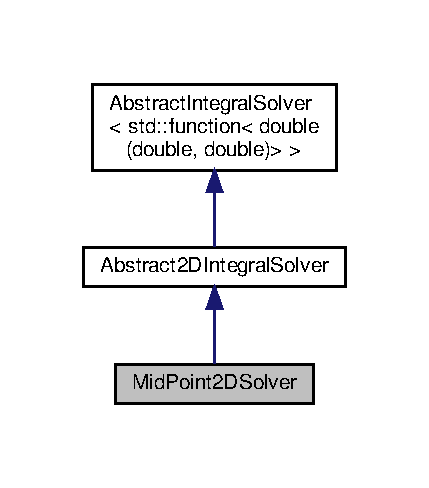
\includegraphics[width=206pt]{class_mid_point2_d_solver__inherit__graph}
\end{center}
\end{figure}


Collaboration diagram for Mid\+Point2\+D\+Solver\+:
\nopagebreak
\begin{figure}[H]
\begin{center}
\leavevmode
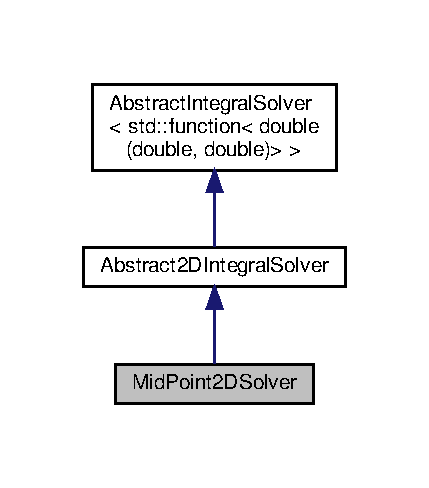
\includegraphics[width=206pt]{class_mid_point2_d_solver__coll__graph}
\end{center}
\end{figure}
\subsection*{Public Types}
\begin{DoxyCompactItemize}
\item 
using \hyperlink{class_mid_point2_d_solver_a1f2d1dcde9b60f07f70d3e8581635714}{t} = std\+::function$<$ double(double, double)$>$
\end{DoxyCompactItemize}
\subsection*{Public Member Functions}
\begin{DoxyCompactItemize}
\item 
\hyperlink{class_mid_point2_d_solver_a9cc9f211031ce410a2fe5287db720460}{Mid\+Point2\+D\+Solver} (int n\+\_\+x, double x0, double xf, int n\+\_\+y, double y0, double yf, \hyperlink{class_mid_point2_d_solver_a1f2d1dcde9b60f07f70d3e8581635714}{t} f)
\item 
double \hyperlink{class_mid_point2_d_solver_a45c6c6802b7d40c35f1f60f1a39f5042}{Solve\+Integral} () override
\end{DoxyCompactItemize}
\subsection*{Additional Inherited Members}


\subsection{Detailed Description}
Daughter Class of \hyperlink{class_abstract2_d_integral_solver}{Abstract2\+D\+Integral\+Solver} which computes a 2D integral using the Midpoint2D method. The Midpoint2D algorithm takes the function value in the middle of the square of length h\+\_\+x and h\+\_\+y. 

\subsection{Member Typedef Documentation}
\mbox{\Hypertarget{class_mid_point2_d_solver_a1f2d1dcde9b60f07f70d3e8581635714}\label{class_mid_point2_d_solver_a1f2d1dcde9b60f07f70d3e8581635714}} 
\index{Mid\+Point2\+D\+Solver@{Mid\+Point2\+D\+Solver}!t@{t}}
\index{t@{t}!Mid\+Point2\+D\+Solver@{Mid\+Point2\+D\+Solver}}
\subsubsection{\texorpdfstring{t}{t}}
{\footnotesize\ttfamily using \hyperlink{class_mid_point2_d_solver_a1f2d1dcde9b60f07f70d3e8581635714}{Mid\+Point2\+D\+Solver\+::t} =  std\+::function$<$double(double, double)$>$}

namespace t is defined as a function which takes two double as an input and returns a double. 

\subsection{Constructor \& Destructor Documentation}
\mbox{\Hypertarget{class_mid_point2_d_solver_a9cc9f211031ce410a2fe5287db720460}\label{class_mid_point2_d_solver_a9cc9f211031ce410a2fe5287db720460}} 
\index{Mid\+Point2\+D\+Solver@{Mid\+Point2\+D\+Solver}!Mid\+Point2\+D\+Solver@{Mid\+Point2\+D\+Solver}}
\index{Mid\+Point2\+D\+Solver@{Mid\+Point2\+D\+Solver}!Mid\+Point2\+D\+Solver@{Mid\+Point2\+D\+Solver}}
\subsubsection{\texorpdfstring{Mid\+Point2\+D\+Solver()}{MidPoint2DSolver()}}
{\footnotesize\ttfamily Mid\+Point2\+D\+Solver\+::\+Mid\+Point2\+D\+Solver (\begin{DoxyParamCaption}\item[{int}]{n\+\_\+x,  }\item[{double}]{x0,  }\item[{double}]{xf,  }\item[{int}]{n\+\_\+y,  }\item[{double}]{y0,  }\item[{double}]{yf,  }\item[{\hyperlink{class_mid_point2_d_solver_a1f2d1dcde9b60f07f70d3e8581635714}{t}}]{f }\end{DoxyParamCaption})\hspace{0.3cm}{\ttfamily [inline]}}

Constructor for \hyperlink{class_mid_point2_d_solver}{Mid\+Point2\+D\+Solver} inherited of \hyperlink{class_abstract2_d_integral_solver}{Abstract2\+D\+Integral\+Solver} 
\begin{DoxyParams}{Parameters}
{\em n\+\_\+x} & number of steps in the x direction \\
\hline
{\em x0} & the beginning of the x interval \\
\hline
{\em xf} & the end of the x interval \\
\hline
{\em n\+\_\+y} & number of steps in the y direction \\
\hline
{\em y0} & the beginning of the y interval \\
\hline
{\em yf} & the end of the y interval \\
\hline
{\em f} & function to integrate dependent on x and y \\
\hline
\end{DoxyParams}


\subsection{Member Function Documentation}
\mbox{\Hypertarget{class_mid_point2_d_solver_a45c6c6802b7d40c35f1f60f1a39f5042}\label{class_mid_point2_d_solver_a45c6c6802b7d40c35f1f60f1a39f5042}} 
\index{Mid\+Point2\+D\+Solver@{Mid\+Point2\+D\+Solver}!Solve\+Integral@{Solve\+Integral}}
\index{Solve\+Integral@{Solve\+Integral}!Mid\+Point2\+D\+Solver@{Mid\+Point2\+D\+Solver}}
\subsubsection{\texorpdfstring{Solve\+Integral()}{SolveIntegral()}}
{\footnotesize\ttfamily double Mid\+Point2\+D\+Solver\+::\+Solve\+Integral (\begin{DoxyParamCaption}{ }\end{DoxyParamCaption})\hspace{0.3cm}{\ttfamily [override]}, {\ttfamily [virtual]}}

Overridden virtual function to solve the integral for the 2D midpoint method \begin{DoxyReturn}{Returns}
the calculated integral of f over the rectangular 2D domain 
\end{DoxyReturn}


Implements \hyperlink{class_abstract_integral_solver}{Abstract\+Integral\+Solver$<$ std\+::function$<$ double(double, double)$>$ $>$}.



The documentation for this class was generated from the following files\+:\begin{DoxyCompactItemize}
\item 
Mid\+Point2\+D\+Solver.\+h\item 
Mid\+Point2\+D\+Solver.\+cpp\end{DoxyCompactItemize}

\hypertarget{class_mid_point_solver}{}\section{Mid\+Point\+Solver Class Reference}
\label{class_mid_point_solver}\index{Mid\+Point\+Solver@{Mid\+Point\+Solver}}


{\ttfamily \#include $<$Mid\+Point\+Solver.\+hpp$>$}



Inheritance diagram for Mid\+Point\+Solver\+:
\nopagebreak
\begin{figure}[H]
\begin{center}
\leavevmode
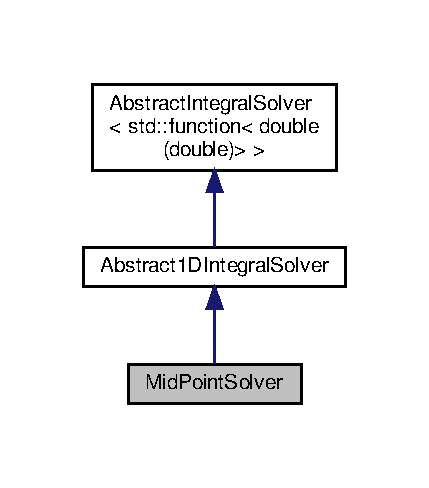
\includegraphics[width=206pt]{class_mid_point_solver__inherit__graph}
\end{center}
\end{figure}


Collaboration diagram for Mid\+Point\+Solver\+:
\nopagebreak
\begin{figure}[H]
\begin{center}
\leavevmode
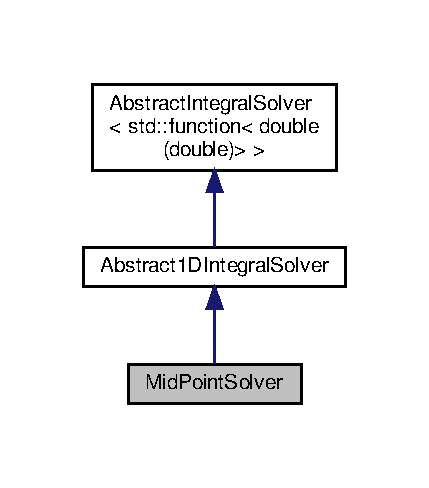
\includegraphics[width=206pt]{class_mid_point_solver__coll__graph}
\end{center}
\end{figure}
\subsection*{Public Types}
\begin{DoxyCompactItemize}
\item 
using \hyperlink{class_mid_point_solver_a48db3b6c36d4edf214150e267c3d063c}{t} = std\+::function$<$ double(double)$>$
\end{DoxyCompactItemize}
\subsection*{Public Member Functions}
\begin{DoxyCompactItemize}
\item 
\hyperlink{class_mid_point_solver_afc0c085bfd86c3f17cb6dd0852ab7426}{Mid\+Point\+Solver} (int n, double x0, double xf, \hyperlink{class_abstract1_d_integral_solver_a7d8e60dfe7eb70e5c19dd71ac0b03880}{t} f)
\item 
double \hyperlink{class_mid_point_solver_a3e7224a0fb07b3ef7f5f9e7e577216cf}{Solve\+Integral} () override
\end{DoxyCompactItemize}
\subsection*{Additional Inherited Members}


\subsection{Detailed Description}
Daughter Class of \hyperlink{class_abstract1_d_integral_solver}{Abstract1\+D\+Integral\+Solver} which computes a 1D integral using the midpoint method. The Midpoint1D algorithm takes the function value in the middle of the sub interval of length h\+\_\+x. 

\subsection{Member Typedef Documentation}
\mbox{\Hypertarget{class_mid_point_solver_a48db3b6c36d4edf214150e267c3d063c}\label{class_mid_point_solver_a48db3b6c36d4edf214150e267c3d063c}} 
\index{Mid\+Point\+Solver@{Mid\+Point\+Solver}!t@{t}}
\index{t@{t}!Mid\+Point\+Solver@{Mid\+Point\+Solver}}
\subsubsection{\texorpdfstring{t}{t}}
{\footnotesize\ttfamily using \hyperlink{class_mid_point_solver_a48db3b6c36d4edf214150e267c3d063c}{Mid\+Point\+Solver\+::t} =  std\+::function$<$double(double)$>$}

namespace t is defined as a function which takes a double as an input and returns a double. 

\subsection{Constructor \& Destructor Documentation}
\mbox{\Hypertarget{class_mid_point_solver_afc0c085bfd86c3f17cb6dd0852ab7426}\label{class_mid_point_solver_afc0c085bfd86c3f17cb6dd0852ab7426}} 
\index{Mid\+Point\+Solver@{Mid\+Point\+Solver}!Mid\+Point\+Solver@{Mid\+Point\+Solver}}
\index{Mid\+Point\+Solver@{Mid\+Point\+Solver}!Mid\+Point\+Solver@{Mid\+Point\+Solver}}
\subsubsection{\texorpdfstring{Mid\+Point\+Solver()}{MidPointSolver()}}
{\footnotesize\ttfamily Mid\+Point\+Solver\+::\+Mid\+Point\+Solver (\begin{DoxyParamCaption}\item[{int}]{n,  }\item[{double}]{x0,  }\item[{double}]{xf,  }\item[{\hyperlink{class_abstract1_d_integral_solver_a7d8e60dfe7eb70e5c19dd71ac0b03880}{t}}]{f }\end{DoxyParamCaption})\hspace{0.3cm}{\ttfamily [inline]}}

Constructor for \hyperlink{class_mid_point_solver}{Mid\+Point\+Solver} inherited of \hyperlink{class_abstract1_d_integral_solver}{Abstract1\+D\+Integral\+Solver} 
\begin{DoxyParams}{Parameters}
{\em n} & number of steps in the x direction \\
\hline
{\em x0} & the beginning of the x interval \\
\hline
{\em xf} & the end of the x interval \\
\hline
{\em f} & function to integrate dependent on x \\
\hline
\end{DoxyParams}


\subsection{Member Function Documentation}
\mbox{\Hypertarget{class_mid_point_solver_a3e7224a0fb07b3ef7f5f9e7e577216cf}\label{class_mid_point_solver_a3e7224a0fb07b3ef7f5f9e7e577216cf}} 
\index{Mid\+Point\+Solver@{Mid\+Point\+Solver}!Solve\+Integral@{Solve\+Integral}}
\index{Solve\+Integral@{Solve\+Integral}!Mid\+Point\+Solver@{Mid\+Point\+Solver}}
\subsubsection{\texorpdfstring{Solve\+Integral()}{SolveIntegral()}}
{\footnotesize\ttfamily double Mid\+Point\+Solver\+::\+Solve\+Integral (\begin{DoxyParamCaption}{ }\end{DoxyParamCaption})\hspace{0.3cm}{\ttfamily [override]}, {\ttfamily [virtual]}}

Overridden virtual function to solve the integral for the 1D midpoint method \begin{DoxyReturn}{Returns}
the calculated integral of f over the interval \mbox{[}x0, xf\mbox{]} 
\end{DoxyReturn}


Implements \hyperlink{class_abstract_integral_solver_ad87cb44c5ef3122bc95be48f473ba399}{Abstract\+Integral\+Solver$<$ std\+::function$<$ double(double)$>$ $>$}.



The documentation for this class was generated from the following files\+:\begin{DoxyCompactItemize}
\item 
Mid\+Point\+Solver.\+hpp\item 
Mid\+Point\+Solver.\+cpp\end{DoxyCompactItemize}

\hypertarget{class_simpson2_d_solver}{}\section{Simpson2\+D\+Solver Class Reference}
\label{class_simpson2_d_solver}\index{Simpson2\+D\+Solver@{Simpson2\+D\+Solver}}


{\ttfamily \#include $<$Simpson2\+D\+Solver.\+h$>$}



Inheritance diagram for Simpson2\+D\+Solver\+:
\nopagebreak
\begin{figure}[H]
\begin{center}
\leavevmode
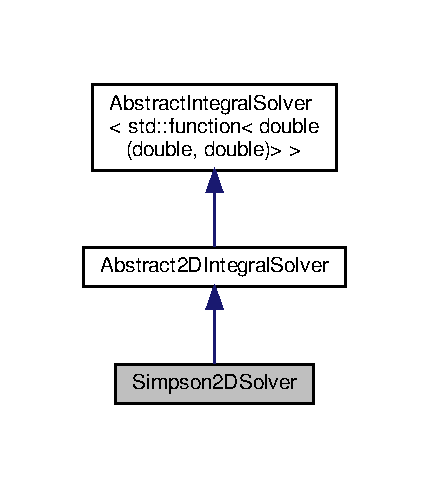
\includegraphics[width=206pt]{class_simpson2_d_solver__inherit__graph}
\end{center}
\end{figure}


Collaboration diagram for Simpson2\+D\+Solver\+:
\nopagebreak
\begin{figure}[H]
\begin{center}
\leavevmode
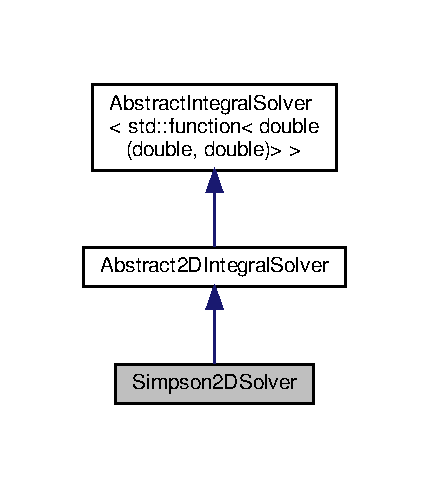
\includegraphics[width=206pt]{class_simpson2_d_solver__coll__graph}
\end{center}
\end{figure}
\subsection*{Public Types}
\begin{DoxyCompactItemize}
\item 
using \hyperlink{class_simpson2_d_solver_a0267d4b1dec3215e954667b1699e687f}{t} = std\+::function$<$ double(double, double)$>$
\end{DoxyCompactItemize}
\subsection*{Public Member Functions}
\begin{DoxyCompactItemize}
\item 
\hyperlink{class_simpson2_d_solver_a16ade6b2b5e89031c452f11e70c2f8fb}{Simpson2\+D\+Solver} (int n\+\_\+x, double x0, double xf, int n\+\_\+y, double y0, double yf, \hyperlink{class_simpson2_d_solver_a0267d4b1dec3215e954667b1699e687f}{t} f)
\item 
double \hyperlink{class_simpson2_d_solver_a3fc19037fef83ad05381138d9f7da939}{Solve\+Integral} () override
\end{DoxyCompactItemize}
\subsection*{Additional Inherited Members}


\subsection{Detailed Description}
Daughter Class of \hyperlink{class_abstract2_d_integral_solver}{Abstract2\+D\+Integral\+Solver} which computes a 2D integral using the Simpson2D method. The Simpson2D algorithm considers several values of the function and gives them different weights. 

\subsection{Member Typedef Documentation}
\mbox{\Hypertarget{class_simpson2_d_solver_a0267d4b1dec3215e954667b1699e687f}\label{class_simpson2_d_solver_a0267d4b1dec3215e954667b1699e687f}} 
\index{Simpson2\+D\+Solver@{Simpson2\+D\+Solver}!t@{t}}
\index{t@{t}!Simpson2\+D\+Solver@{Simpson2\+D\+Solver}}
\subsubsection{\texorpdfstring{t}{t}}
{\footnotesize\ttfamily using \hyperlink{class_simpson2_d_solver_a0267d4b1dec3215e954667b1699e687f}{Simpson2\+D\+Solver\+::t} =  std\+::function$<$double(double, double)$>$}

namespace t is defined as a function which takes two doubles as an input and returns a double. 

\subsection{Constructor \& Destructor Documentation}
\mbox{\Hypertarget{class_simpson2_d_solver_a16ade6b2b5e89031c452f11e70c2f8fb}\label{class_simpson2_d_solver_a16ade6b2b5e89031c452f11e70c2f8fb}} 
\index{Simpson2\+D\+Solver@{Simpson2\+D\+Solver}!Simpson2\+D\+Solver@{Simpson2\+D\+Solver}}
\index{Simpson2\+D\+Solver@{Simpson2\+D\+Solver}!Simpson2\+D\+Solver@{Simpson2\+D\+Solver}}
\subsubsection{\texorpdfstring{Simpson2\+D\+Solver()}{Simpson2DSolver()}}
{\footnotesize\ttfamily Simpson2\+D\+Solver\+::\+Simpson2\+D\+Solver (\begin{DoxyParamCaption}\item[{int}]{n\+\_\+x,  }\item[{double}]{x0,  }\item[{double}]{xf,  }\item[{int}]{n\+\_\+y,  }\item[{double}]{y0,  }\item[{double}]{yf,  }\item[{\hyperlink{class_simpson2_d_solver_a0267d4b1dec3215e954667b1699e687f}{t}}]{f }\end{DoxyParamCaption})\hspace{0.3cm}{\ttfamily [inline]}}

Constructor for \hyperlink{class_simpson2_d_solver}{Simpson2\+D\+Solver} inherited of \hyperlink{class_abstract2_d_integral_solver}{Abstract2\+D\+Integral\+Solver} 
\begin{DoxyParams}{Parameters}
{\em n\+\_\+x} & number of steps in the x direction \\
\hline
{\em x0} & the beginning of the x interval \\
\hline
{\em xf} & the end of the x interval \\
\hline
{\em n\+\_\+y} & number of steps in the y direction \\
\hline
{\em y0} & the beginning of the y interval \\
\hline
{\em yf} & the end of the y interval \\
\hline
{\em f} & function to integrate dependent on x and y \\
\hline
\end{DoxyParams}


\subsection{Member Function Documentation}
\mbox{\Hypertarget{class_simpson2_d_solver_a3fc19037fef83ad05381138d9f7da939}\label{class_simpson2_d_solver_a3fc19037fef83ad05381138d9f7da939}} 
\index{Simpson2\+D\+Solver@{Simpson2\+D\+Solver}!Solve\+Integral@{Solve\+Integral}}
\index{Solve\+Integral@{Solve\+Integral}!Simpson2\+D\+Solver@{Simpson2\+D\+Solver}}
\subsubsection{\texorpdfstring{Solve\+Integral()}{SolveIntegral()}}
{\footnotesize\ttfamily double Simpson2\+D\+Solver\+::\+Solve\+Integral (\begin{DoxyParamCaption}{ }\end{DoxyParamCaption})\hspace{0.3cm}{\ttfamily [override]}, {\ttfamily [virtual]}}

Overridden virtual function to solve the integral for the 2D simpson method \begin{DoxyReturn}{Returns}
the calculated integral of f over the rectangular 2D domain 
\end{DoxyReturn}


Implements \hyperlink{class_abstract_integral_solver}{Abstract\+Integral\+Solver$<$ std\+::function$<$ double(double, double)$>$ $>$}.



The documentation for this class was generated from the following files\+:\begin{DoxyCompactItemize}
\item 
Simpson2\+D\+Solver.\+h\item 
Simpson2\+D\+Solver.\+cpp\end{DoxyCompactItemize}

\hypertarget{class_simpson_solver}{}\section{Simpson\+Solver Class Reference}
\label{class_simpson_solver}\index{Simpson\+Solver@{Simpson\+Solver}}


{\ttfamily \#include $<$Simpson\+Solver.\+hpp$>$}



Inheritance diagram for Simpson\+Solver\+:\nopagebreak
\begin{figure}[H]
\begin{center}
\leavevmode
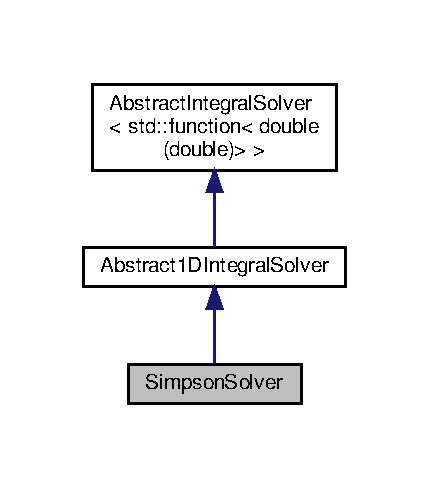
\includegraphics[width=206pt]{class_simpson_solver__inherit__graph}
\end{center}
\end{figure}


Collaboration diagram for Simpson\+Solver\+:\nopagebreak
\begin{figure}[H]
\begin{center}
\leavevmode
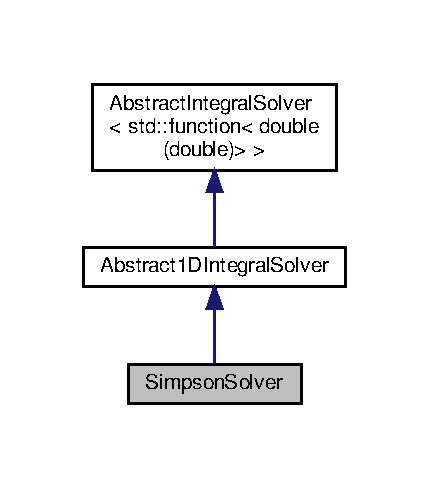
\includegraphics[width=206pt]{class_simpson_solver__coll__graph}
\end{center}
\end{figure}
\subsection*{Public Types}
\begin{DoxyCompactItemize}
\item 
using \hyperlink{class_simpson_solver_aa31ea3c884d669836ba1d0399aa53479}{t} = std\+::function$<$ double(double)$>$
\end{DoxyCompactItemize}
\subsection*{Public Member Functions}
\begin{DoxyCompactItemize}
\item 
\hyperlink{class_simpson_solver_abc9059969016bce44332013d48baeed2}{Simpson\+Solver} (int n, double x0, double xf, \hyperlink{class_abstract1_d_integral_solver_a7d8e60dfe7eb70e5c19dd71ac0b03880}{t} f)
\item 
double \hyperlink{class_simpson_solver_a4843e8bfc0344d9a9cae8688d1114667}{Solve\+Integral} () override
\end{DoxyCompactItemize}
\subsection*{Additional Inherited Members}


\subsection{Detailed Description}
Daughter Class of \hyperlink{class_abstract1_d_integral_solver}{Abstract1\+D\+Integral\+Solver} which computes a 1D integral using the Simpson2D method. The Simpson2D algorithm considers the extreme points of the sub interval with weight 1 and the middle of the sub interval with weight 4. 

\subsection{Member Typedef Documentation}
\mbox{\Hypertarget{class_simpson_solver_aa31ea3c884d669836ba1d0399aa53479}\label{class_simpson_solver_aa31ea3c884d669836ba1d0399aa53479}} 
\index{Simpson\+Solver@{Simpson\+Solver}!t@{t}}
\index{t@{t}!Simpson\+Solver@{Simpson\+Solver}}
\subsubsection{\texorpdfstring{t}{t}}
{\footnotesize\ttfamily using \hyperlink{class_simpson_solver_aa31ea3c884d669836ba1d0399aa53479}{Simpson\+Solver\+::t} =  std\+::function$<$double(double)$>$}

namespace t is defined as a function which takes a double as an input and returns a double. 

\subsection{Constructor \& Destructor Documentation}
\mbox{\Hypertarget{class_simpson_solver_abc9059969016bce44332013d48baeed2}\label{class_simpson_solver_abc9059969016bce44332013d48baeed2}} 
\index{Simpson\+Solver@{Simpson\+Solver}!Simpson\+Solver@{Simpson\+Solver}}
\index{Simpson\+Solver@{Simpson\+Solver}!Simpson\+Solver@{Simpson\+Solver}}
\subsubsection{\texorpdfstring{Simpson\+Solver()}{SimpsonSolver()}}
{\footnotesize\ttfamily Simpson\+Solver\+::\+Simpson\+Solver (\begin{DoxyParamCaption}\item[{int}]{n,  }\item[{double}]{x0,  }\item[{double}]{xf,  }\item[{\hyperlink{class_abstract1_d_integral_solver_a7d8e60dfe7eb70e5c19dd71ac0b03880}{t}}]{f }\end{DoxyParamCaption})\hspace{0.3cm}{\ttfamily [inline]}}

Constructor for \hyperlink{class_simpson_solver}{Simpson\+Solver} inherited of \hyperlink{class_abstract1_d_integral_solver}{Abstract1\+D\+Integral\+Solver} 
\begin{DoxyParams}{Parameters}
{\em n} & number of steps in the x direction \\
\hline
{\em x0} & the beginning of the x interval \\
\hline
{\em xf} & the end of the x interval \\
\hline
{\em f} & function to integrate over the interval \mbox{[}x0, xf\mbox{]} dependent on x \\
\hline
\end{DoxyParams}


\subsection{Member Function Documentation}
\mbox{\Hypertarget{class_simpson_solver_a4843e8bfc0344d9a9cae8688d1114667}\label{class_simpson_solver_a4843e8bfc0344d9a9cae8688d1114667}} 
\index{Simpson\+Solver@{Simpson\+Solver}!Solve\+Integral@{Solve\+Integral}}
\index{Solve\+Integral@{Solve\+Integral}!Simpson\+Solver@{Simpson\+Solver}}
\subsubsection{\texorpdfstring{Solve\+Integral()}{SolveIntegral()}}
{\footnotesize\ttfamily double Simpson\+Solver\+::\+Solve\+Integral (\begin{DoxyParamCaption}{ }\end{DoxyParamCaption})\hspace{0.3cm}{\ttfamily [override]}, {\ttfamily [virtual]}}

Overridden virtual function to solve the integral for the 1D simpson method \begin{DoxyReturn}{Returns}
the calculated integral of f over the interval \mbox{[}x0, xf\mbox{]} 
\end{DoxyReturn}


Implements \hyperlink{class_abstract_integral_solver_ad87cb44c5ef3122bc95be48f473ba399}{Abstract\+Integral\+Solver$<$ std\+::function$<$ double(double)$>$ $>$}.



The documentation for this class was generated from the following files\+:\begin{DoxyCompactItemize}
\item 
Simpson\+Solver.\+hpp\item 
Simpson\+Solver.\+cpp\end{DoxyCompactItemize}

\hypertarget{classtest_suite1_d}{}\section{test\+Suite1D Class Reference}
\label{classtest_suite1_d}\index{test\+Suite1D@{test\+Suite1D}}


The documentation for this class was generated from the following file\+:\begin{DoxyCompactItemize}
\item 
test\+Suite.\+h\end{DoxyCompactItemize}

\hypertarget{class_trapez2_d_solver}{}\section{Trapez2\+D\+Solver Class Reference}
\label{class_trapez2_d_solver}\index{Trapez2\+D\+Solver@{Trapez2\+D\+Solver}}


Inheritance diagram for Trapez2\+D\+Solver\+:
\nopagebreak
\begin{figure}[H]
\begin{center}
\leavevmode
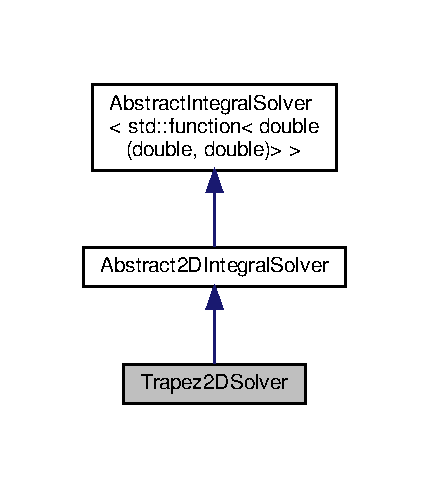
\includegraphics[width=206pt]{class_trapez2_d_solver__inherit__graph}
\end{center}
\end{figure}


Collaboration diagram for Trapez2\+D\+Solver\+:
\nopagebreak
\begin{figure}[H]
\begin{center}
\leavevmode
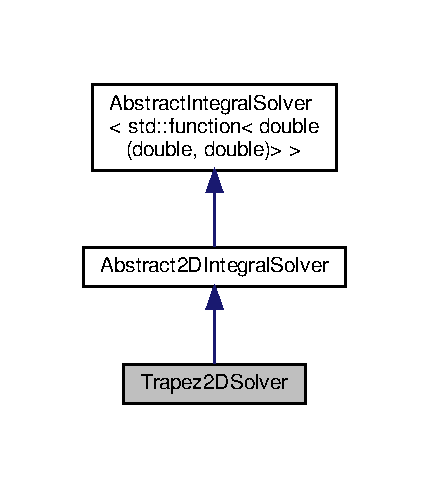
\includegraphics[width=206pt]{class_trapez2_d_solver__coll__graph}
\end{center}
\end{figure}
\subsection*{Public Types}
\begin{DoxyCompactItemize}
\item 
\mbox{\Hypertarget{class_trapez2_d_solver_a2af165a7995664482df24eec24a39ec3}\label{class_trapez2_d_solver_a2af165a7995664482df24eec24a39ec3}} 
using {\bfseries t} = std\+::function$<$ double(double, double)$>$
\end{DoxyCompactItemize}
\subsection*{Public Member Functions}
\begin{DoxyCompactItemize}
\item 
\mbox{\Hypertarget{class_trapez2_d_solver_a95b57f9279e40991610b4e91747d7e0d}\label{class_trapez2_d_solver_a95b57f9279e40991610b4e91747d7e0d}} 
{\bfseries Trapez2\+D\+Solver} (int n\+\_\+x, double x0, double xf, int n\+\_\+y, double y0, double yf, t f)
\item 
\mbox{\Hypertarget{class_trapez2_d_solver_a88f724ff6fd2c566d54f5d0ccc500cb9}\label{class_trapez2_d_solver_a88f724ff6fd2c566d54f5d0ccc500cb9}} 
double {\bfseries Solve\+Integral} () override
\end{DoxyCompactItemize}
\subsection*{Additional Inherited Members}


The documentation for this class was generated from the following files\+:\begin{DoxyCompactItemize}
\item 
Trapez2\+D\+Solver.\+h\item 
Trapez2\+D\+Solver.\+cpp\end{DoxyCompactItemize}

\hypertarget{class_trapez_solver}{}\section{Trapez\+Solver Class Reference}
\label{class_trapez_solver}\index{Trapez\+Solver@{Trapez\+Solver}}


{\ttfamily \#include $<$Trapez\+Solver.\+hpp$>$}



Inheritance diagram for Trapez\+Solver\+:\nopagebreak
\begin{figure}[H]
\begin{center}
\leavevmode
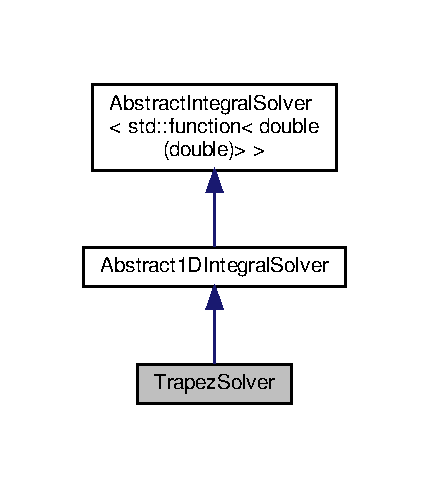
\includegraphics[width=206pt]{class_trapez_solver__inherit__graph}
\end{center}
\end{figure}


Collaboration diagram for Trapez\+Solver\+:\nopagebreak
\begin{figure}[H]
\begin{center}
\leavevmode
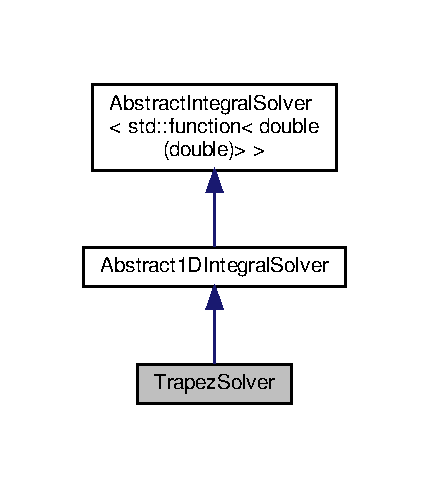
\includegraphics[width=206pt]{class_trapez_solver__coll__graph}
\end{center}
\end{figure}
\subsection*{Public Types}
\begin{DoxyCompactItemize}
\item 
using \hyperlink{class_trapez_solver_ac94a3e89df0d6bacc7d62e3784fd4162}{t} = \hyperlink{_tests_8cpp_a1c2dbde1ba7d93e381d4ccb9f603be16}{std\+::function}$<$ double(double)$>$
\end{DoxyCompactItemize}
\subsection*{Public Member Functions}
\begin{DoxyCompactItemize}
\item 
\hyperlink{class_trapez_solver_aacba017d146636c666dff931f6c43323}{Trapez\+Solver} (int n, double x0, double xf, \hyperlink{class_abstract1_d_integral_solver_a7d8e60dfe7eb70e5c19dd71ac0b03880}{t} f)
\item 
double \hyperlink{class_trapez_solver_a15651e2fba081b87b484a83fc424c81d}{Solve\+Integral} () override
\end{DoxyCompactItemize}
\subsection*{Additional Inherited Members}


\subsection{Detailed Description}
Daughter Class of \hyperlink{class_abstract1_d_integral_solver}{Abstract1\+D\+Integral\+Solver} which computes a 1D integral using the trapezoidal method. The Trapezoidal1D algorithm takes the function values at the extreme points of the sub intervals of length h\+\_\+x. Both points have the same weight. 

\subsection{Member Typedef Documentation}
\mbox{\Hypertarget{class_trapez_solver_ac94a3e89df0d6bacc7d62e3784fd4162}\label{class_trapez_solver_ac94a3e89df0d6bacc7d62e3784fd4162}} 
\index{Trapez\+Solver@{Trapez\+Solver}!t@{t}}
\index{t@{t}!Trapez\+Solver@{Trapez\+Solver}}
\subsubsection{\texorpdfstring{t}{t}}
{\footnotesize\ttfamily using \hyperlink{class_trapez_solver_ac94a3e89df0d6bacc7d62e3784fd4162}{Trapez\+Solver\+::t} =  \hyperlink{_tests_8cpp_a1c2dbde1ba7d93e381d4ccb9f603be16}{std\+::function}$<$double(double)$>$}

namespace t is defined as a function which takes a double as an input and returns a double. 

\subsection{Constructor \& Destructor Documentation}
\mbox{\Hypertarget{class_trapez_solver_aacba017d146636c666dff931f6c43323}\label{class_trapez_solver_aacba017d146636c666dff931f6c43323}} 
\index{Trapez\+Solver@{Trapez\+Solver}!Trapez\+Solver@{Trapez\+Solver}}
\index{Trapez\+Solver@{Trapez\+Solver}!Trapez\+Solver@{Trapez\+Solver}}
\subsubsection{\texorpdfstring{Trapez\+Solver()}{TrapezSolver()}}
{\footnotesize\ttfamily Trapez\+Solver\+::\+Trapez\+Solver (\begin{DoxyParamCaption}\item[{int}]{n,  }\item[{double}]{x0,  }\item[{double}]{xf,  }\item[{\hyperlink{class_abstract1_d_integral_solver_a7d8e60dfe7eb70e5c19dd71ac0b03880}{t}}]{f }\end{DoxyParamCaption})\hspace{0.3cm}{\ttfamily [inline]}}

Constructor for \hyperlink{class_trapez_solver}{Trapez\+Solver} inherited of \hyperlink{class_abstract1_d_integral_solver}{Abstract1\+D\+Integral\+Solver} 
\begin{DoxyParams}{Parameters}
{\em n} & number of steps in the x direction \\
\hline
{\em x0} & the beginning of the x interval \\
\hline
{\em xf} & the end of the x interval \\
\hline
{\em f} & function to integrate dependent on x \\
\hline
\end{DoxyParams}


\subsection{Member Function Documentation}
\mbox{\Hypertarget{class_trapez_solver_a15651e2fba081b87b484a83fc424c81d}\label{class_trapez_solver_a15651e2fba081b87b484a83fc424c81d}} 
\index{Trapez\+Solver@{Trapez\+Solver}!Solve\+Integral@{Solve\+Integral}}
\index{Solve\+Integral@{Solve\+Integral}!Trapez\+Solver@{Trapez\+Solver}}
\subsubsection{\texorpdfstring{Solve\+Integral()}{SolveIntegral()}}
{\footnotesize\ttfamily double Trapez\+Solver\+::\+Solve\+Integral (\begin{DoxyParamCaption}{ }\end{DoxyParamCaption})\hspace{0.3cm}{\ttfamily [override]}, {\ttfamily [virtual]}}

Overridden virtual function to solve the integral for the 1D midpoint method \begin{DoxyReturn}{Returns}
the calculated integral of f over the interval \mbox{[}x0, xf\mbox{]} 
\end{DoxyReturn}


Implements \hyperlink{class_abstract_integral_solver_ad87cb44c5ef3122bc95be48f473ba399}{Abstract\+Integral\+Solver$<$ std\+::function$<$ double(double)$>$ $>$}.



The documentation for this class was generated from the following files\+:\begin{DoxyCompactItemize}
\item 
\hyperlink{_trapez_solver_8hpp}{Trapez\+Solver.\+hpp}\item 
\hyperlink{_trapez_solver_8cpp}{Trapez\+Solver.\+cpp}\end{DoxyCompactItemize}

%--- End generated contents ---

% Index
\backmatter
\newpage
\phantomsection
\clearemptydoublepage
\addcontentsline{toc}{chapter}{Index}
\printindex

\end{document}
